\documentclass[11pt]{article}
\usepackage[margin=1in]{geometry}
\usepackage{amsmath, amssymb, amsfonts}
\usepackage{graphicx}
\usepackage{algorithm}
\usepackage{algpseudocode}
\usepackage{hyperref}
\usepackage{booktabs}
\usepackage{enumitem}
\usepackage{float}
\usepackage{caption}

\title{\textbf{AI 543: Foundation of Online Machine Learning} \\ \textbf{Homework 3: Bandit Algorithms}}
\author{Mrinal Bharadwaj}
\date{March 2, 2026}

\begin{document}
\maketitle

% ============================================================================
% OVERVIEW
% ============================================================================
\section{Overview}

This report presents the implementation and evaluation of classical bandit algorithms in simulated environments. The experiments cover:
\begin{itemize}[noitemsep]
    \item \textbf{Task 1 (Multi-Armed Bandits):} Explore Then Commit, UCB, Thompson Sampling
    \item \textbf{Task 2 (Linear Bandits):} LinUCB, LinTS
\end{itemize}

\noindent All results can be reproduced by running:
\begin{verbatim}
    python RunAll.py
\end{verbatim}

% ============================================================================
% TASK 1: MULTI-ARMED BANDITS
% ============================================================================
\section{Task 1: Multi-Armed Bandits (60 points)}

\subsection{Environment Setup}

To simulate a $K$-armed bandit, we use the following settings:
\begin{itemize}[noitemsep]
    \item \texttt{actionset = "basis\_vector"}: article feature vectors are basis vectors $e_0, e_1, \ldots, e_{K-1}$, making arms independent.
    \item $K = $ \texttt{n\_articles} $ = $ \texttt{context\_dimension} $ = 10$
    \item \texttt{NoiseScale} $= \sigma = 0.1$ (standard deviation of Gaussian noise)
    \item \texttt{n\_users} $= 10$
    \item \texttt{testing\_iterations} $= 10{,}000$
    \item \texttt{poolArticleSize} $=$ None (all arms available each round)
\end{itemize}

Since feature vectors are basis vectors, the reward for arm $i$ selected by user with parameter $\theta$ is:
\[
r_t = \theta^\top e_i + \epsilon_t = \theta_i + \epsilon_t, \quad \epsilon_t \sim \mathcal{N}(0, \sigma^2)
\]
Each arm has an independent mean reward $\mu_i = \theta_i$, which the algorithms must learn.

% ---------- ETC ----------
\subsection{Explore Then Commit (20 points)}

\subsubsection{Algorithm Description}

\textbf{Input:} Number of arms $K$, exploration parameter $m$, arm set $\mathcal{A}$.

\begin{algorithm}[H]
\caption{Explore Then Commit}
\begin{algorithmic}[1]
\State \textbf{Exploration Phase:} For each arm $i \in \{1, \ldots, K\}$, pull arm $i$ exactly $m$ times.
\State Record the empirical mean reward for each arm:
\[
\hat{\mu}_i = \frac{1}{m} \sum_{s=1}^{m} r_{i,s}
\]
\State \textbf{Commit Phase:} For all remaining rounds $t > mK$, always select:
\[
a_t = \arg\max_{i \in \{1,\ldots,K\}} \hat{\mu}_i
\]
\end{algorithmic}
\end{algorithm}

The total exploration phase lasts $m \times K$ rounds. After that, the algorithm commits to the arm with the highest observed mean forever.

\subsubsection{Results}

We test $m \in \{1, 2, 3, 5, 8, 10, 15, 20, 50, 100, 200, 500\}$ (12 values).

\begin{figure}[H]
    \centering
    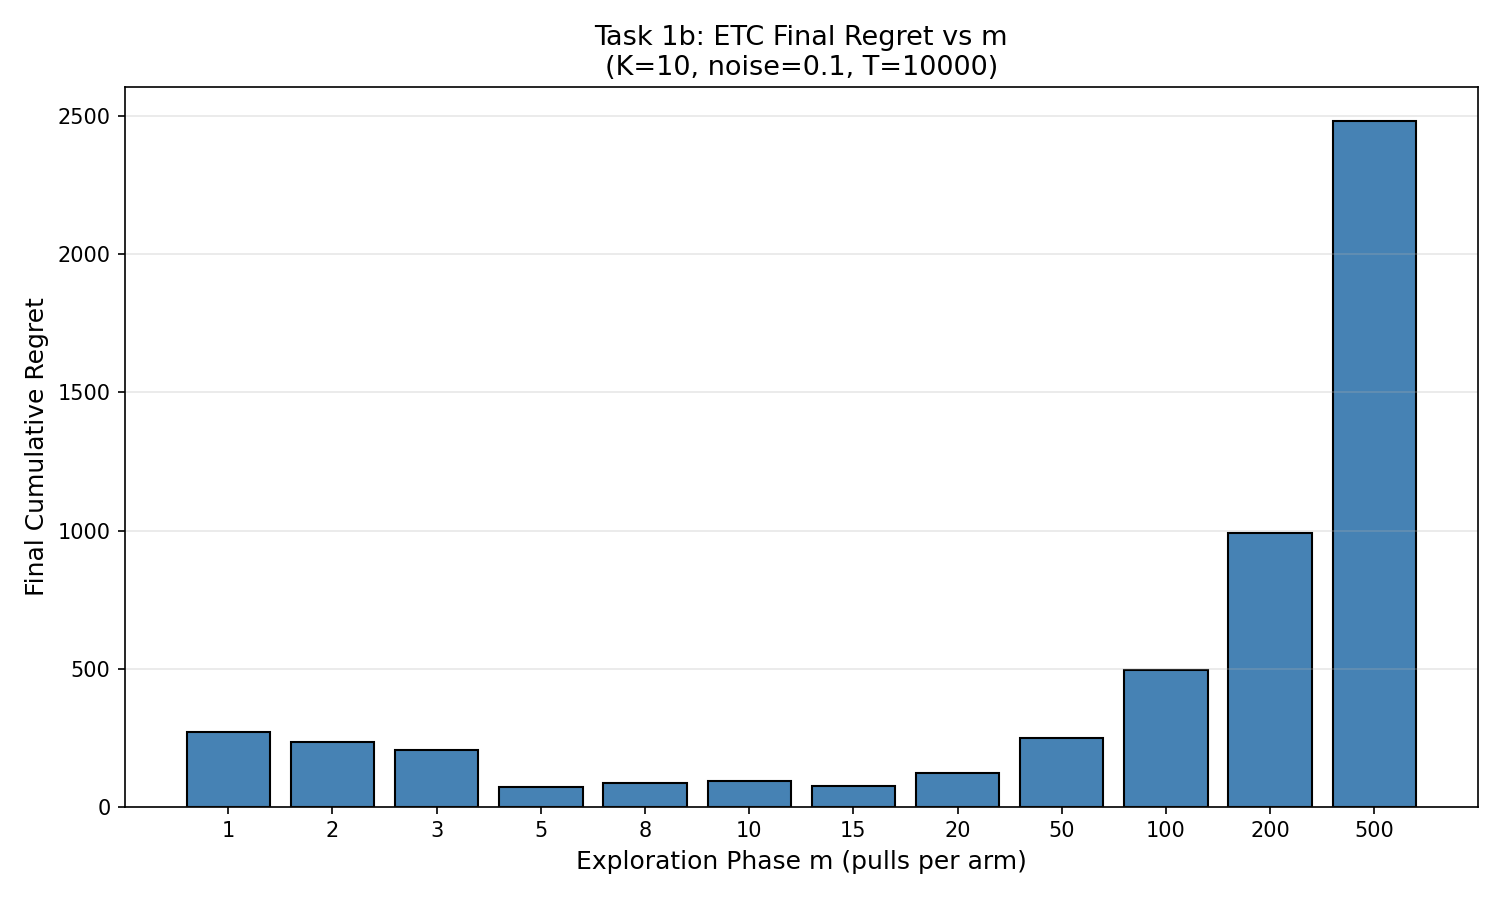
\includegraphics[width=0.85\textwidth]{SimulationResults/Task1b_ETC_regret_vs_m.png}
    \caption{ETC: Final cumulative regret as a function of $m$.}
    \label{fig:etc_bar}
\end{figure}

\begin{figure}[H]
    \centering
    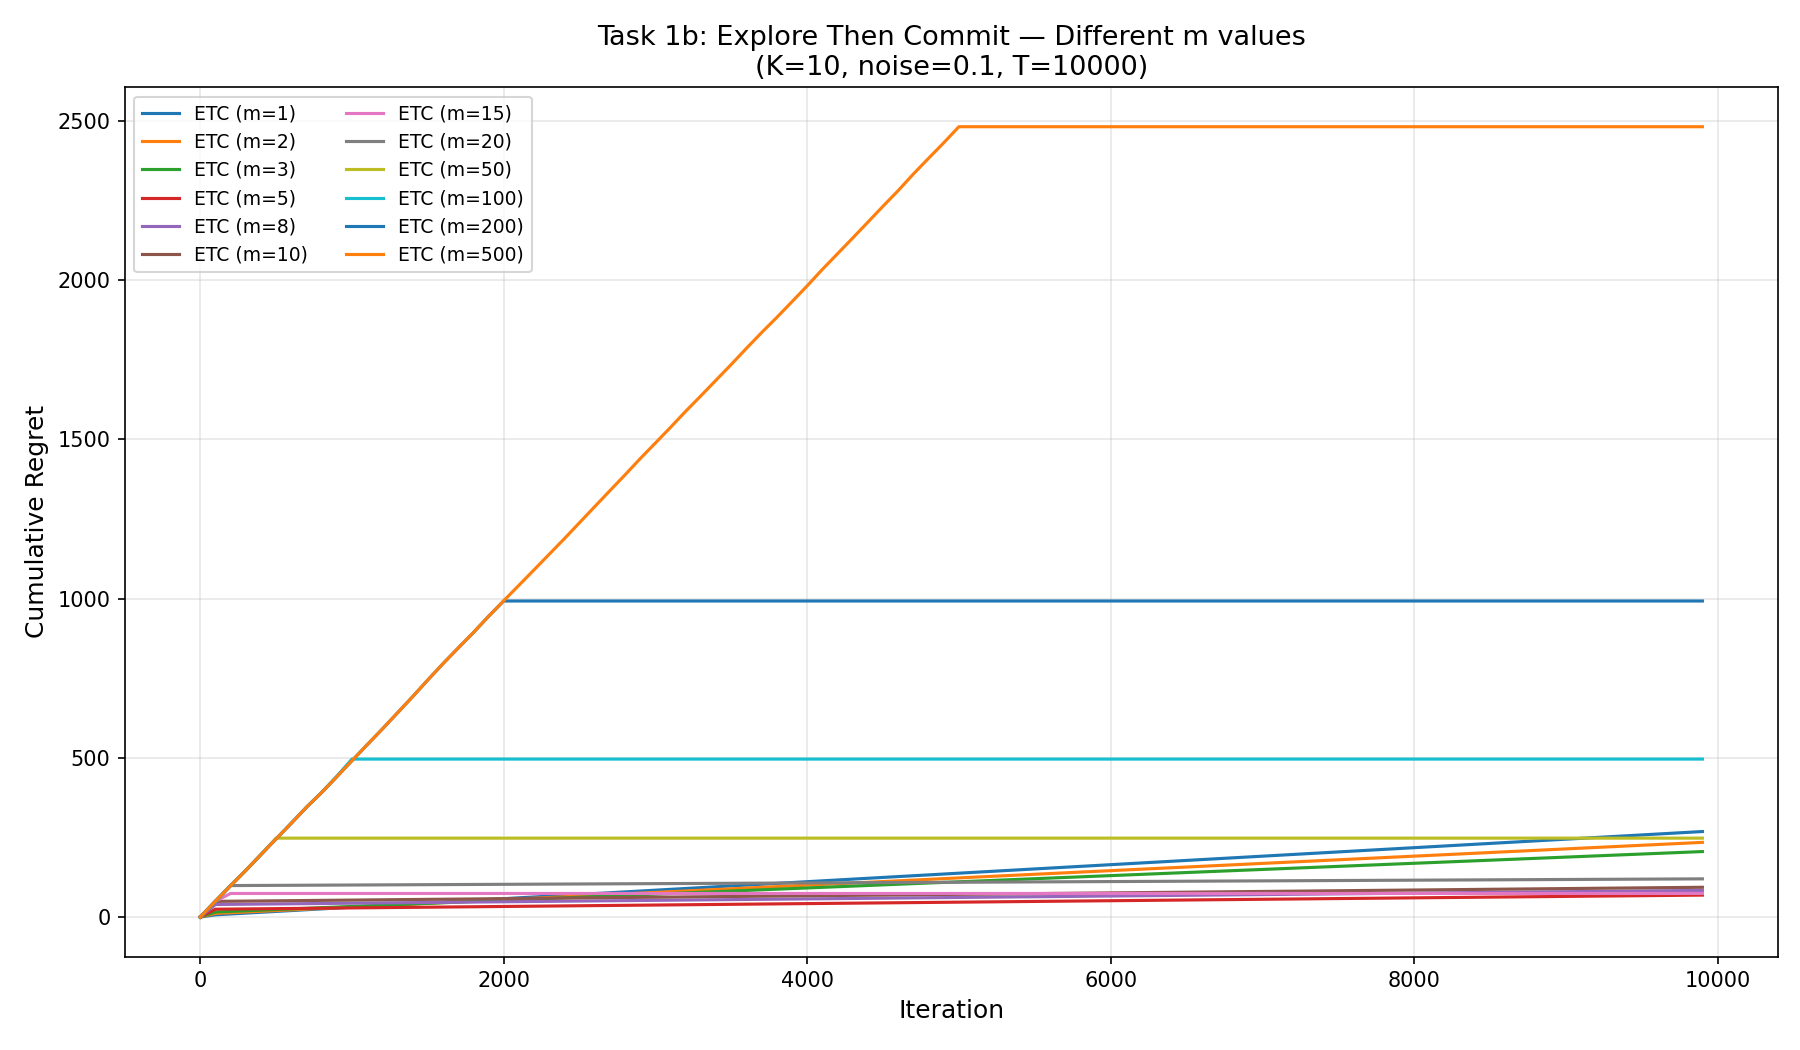
\includegraphics[width=0.85\textwidth]{SimulationResults/Task1b_ETC_all_m.png}
    \caption{ETC: Cumulative regret over time for all $m$ values.}
    \label{fig:etc_curves}
\end{figure}

\begin{table}[H]
\centering
\caption{ETC final cumulative regret for different $m$ values.}
\label{tab:etc}
\begin{tabular}{cc}
\toprule
$m$ (pulls per arm) & Final Cumulative Regret \\
\midrule
1   & 268.91 \\
2   & 234.86 \\
3   & 206.01 \\
\textbf{5}   & \textbf{69.30} \\
8   & 84.05 \\
10  & 93.89 \\
15  & 74.45 \\
20  & 120.30 \\
50  & 248.17 \\
100 & 496.34 \\
200 & 992.68 \\
500 & 2481.69 \\
\bottomrule
\end{tabular}
\end{table}

\subsubsection{Analysis: Which $m$ is best and why?}

The best $m$ is $\mathbf{m = 5}$ with a final cumulative regret of $69.30$. The results show a clear U-shaped tradeoff:

\begin{itemize}
    \item \textbf{$m$ too small} (e.g., $m=1, 2$): Each arm is explored very few times. With noise ($\sigma = 0.1$), the empirical mean $\hat{\mu}_i$ is a poor estimate of the true mean $\mu_i$. The algorithm frequently commits to a \textit{suboptimal} arm, leading to high regret that accumulates linearly forever after the commit phase.
    \item \textbf{$m$ too large} (e.g., $m=100, 200, 500$): The exploration phase itself takes $m \times K$ rounds. With $m = 500$ and $K = 10$, the algorithm spends $5{,}000$ out of $10{,}000$ rounds just exploring, pulling suboptimal arms many times unnecessarily. This wastes rounds that could be spent exploiting the best arm.
    \item \textbf{$m$ just right} ($m \approx 5$): The algorithm gets a sufficiently accurate estimate of each arm's mean (with $m=5$ observations and $\sigma=0.1$, the standard error is $\sigma / \sqrt{m} = 0.045$, which is small enough to distinguish arms) while spending only $50$ rounds exploring.
\end{itemize}

% ---------- UCB ----------
\subsection{UCB (20 points)}

\subsubsection{Algorithm Description}

\textbf{Input:} Number of arms $K$, exploration parameter $\alpha$.

The UCB (Upper Confidence Bound) algorithm selects the arm that maximizes an optimistic estimate of the mean reward. The UCB index for arm $i$ at time $t$ is:

\begin{equation}
\text{UCB}_i(t) = \hat{\mu}_i(t) + \alpha \sqrt{\frac{\ln t}{N_i(t)}}
\label{eq:ucb}
\end{equation}

where:
\begin{itemize}[noitemsep]
    \item $\hat{\mu}_i(t)$ is the empirical mean reward of arm $i$ up to time $t$
    \item $N_i(t)$ is the number of times arm $i$ has been pulled up to time $t$
    \item $t$ is the total number of pulls so far
    \item $\alpha$ is the exploration parameter controlling the width of the confidence bound
\end{itemize}

\begin{algorithm}[H]
\caption{UCB}
\begin{algorithmic}[1]
\State Pull each arm once (initialization).
\For{$t = K+1, K+2, \ldots, T$}
    \State For each arm $i$, compute $\text{UCB}_i(t)$ using Eq.~\eqref{eq:ucb}.
    \State Select $a_t = \arg\max_{i} \text{UCB}_i(t)$.
    \State Observe reward $r_t$ and update $\hat{\mu}_{a_t}$ and $N_{a_t}$.
\EndFor
\end{algorithmic}
\end{algorithm}

The key idea is ``optimism in the face of uncertainty'': arms with fewer observations receive a larger exploration bonus, encouraging the algorithm to try under-explored arms.

\subsubsection{Results}

\begin{figure}[H]
    \centering
    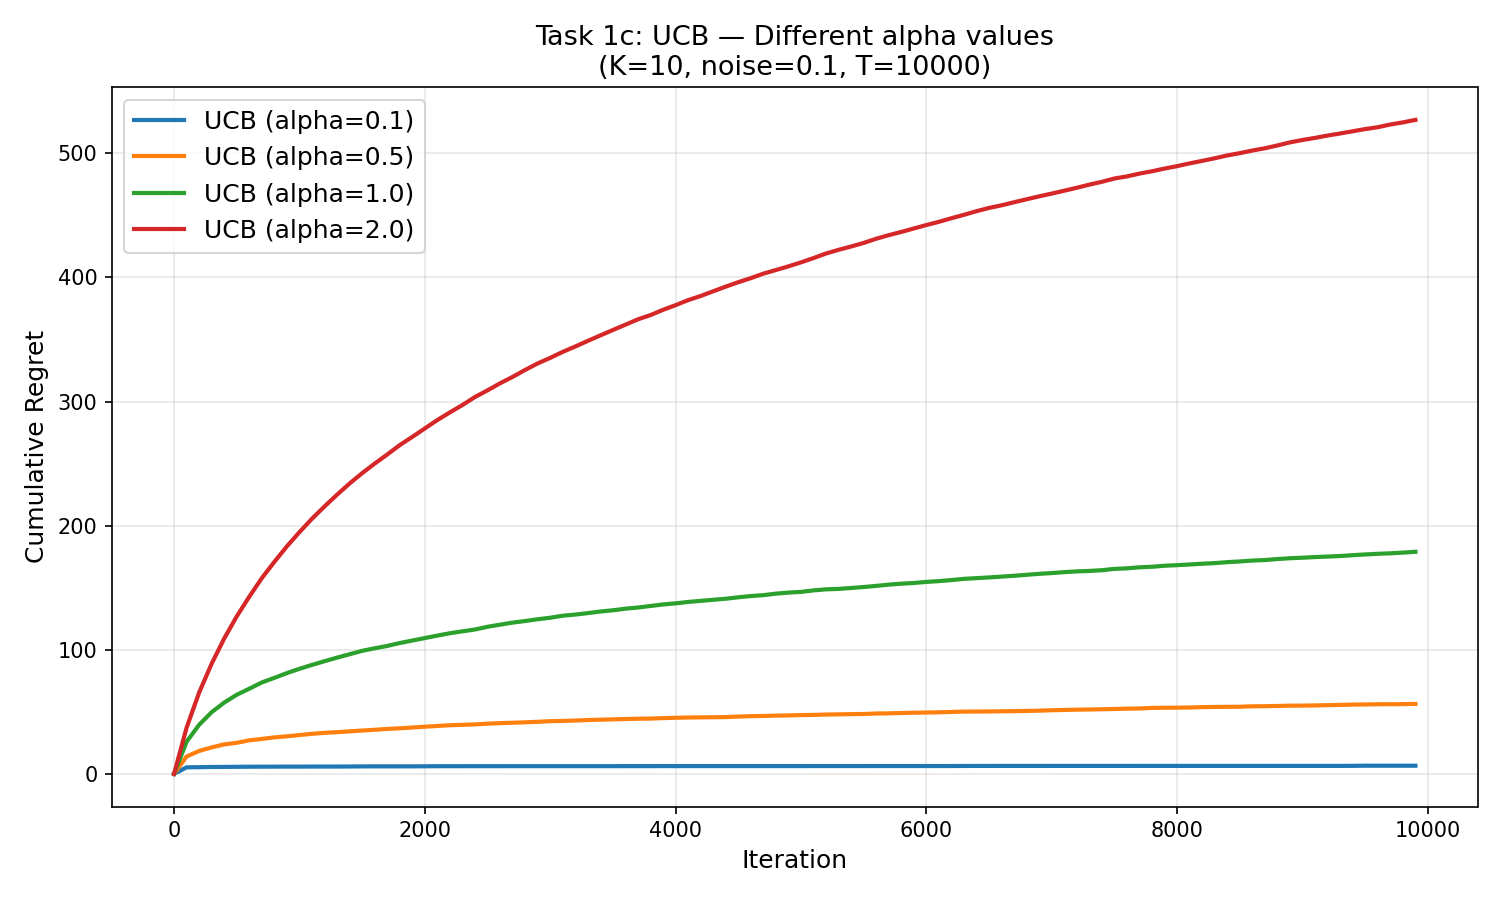
\includegraphics[width=0.85\textwidth]{SimulationResults/Task1c_UCB.png}
    \caption{UCB: Cumulative regret with different $\alpha$ values.}
    \label{fig:ucb}
\end{figure}

\begin{table}[H]
\centering
\caption{UCB final cumulative regret for different $\alpha$ values.}
\begin{tabular}{cc}
\toprule
$\alpha$ & Final Cumulative Regret \\
\midrule
0.1 & 7.02 \\
0.5 & 56.74 \\
1.0 & 179.13 \\
2.0 & 526.61 \\
\bottomrule
\end{tabular}
\end{table}

Smaller $\alpha$ reduces unnecessary exploration. With low noise ($\sigma = 0.1$), the algorithm quickly identifies the best arm and $\alpha = 0.1$ is sufficient. The regret of UCB grows logarithmically $O(\ln T)$, which is visible in the flattening curves.

% ---------- Thompson Sampling ----------
\subsection{Thompson Sampling (20 points)}

\subsubsection{Algorithm Description}

\textbf{Input:} Number of arms $K$, known noise variance $\sigma^2$.

Thompson Sampling uses a Bayesian approach. We maintain a posterior distribution over each arm's mean reward $\mu_i$ and sample from it to make decisions.

\textbf{Prior:}
\[
\mu_i \sim \mathcal{N}(0, 1) \quad \text{for each arm } i
\]

\textbf{Likelihood:}
\[
r_t \mid \mu_i \sim \mathcal{N}(\mu_i, \sigma^2)
\]

\textbf{Posterior} after observing $n_i$ rewards with sum $S_i = \sum_{s=1}^{n_i} r_{i,s}$:
\begin{align}
\tau_i^2 &= \frac{1}{\frac{1}{\sigma_0^2} + \frac{n_i}{\sigma^2}} \label{eq:ts_var} \\
m_i &= \tau_i^2 \left( \frac{\mu_0}{\sigma_0^2} + \frac{S_i}{\sigma^2} \right) \label{eq:ts_mean} \\
\mu_i \mid \text{data} &\sim \mathcal{N}(m_i, \tau_i^2)
\end{align}
where $\mu_0 = 0$ and $\sigma_0^2 = 1$ are the prior mean and variance.

\begin{algorithm}[H]
\caption{Thompson Sampling (Gaussian)}
\begin{algorithmic}[1]
\For{$t = 1, 2, \ldots, T$}
    \For{each arm $i$ in the available set}
        \State Compute posterior mean $m_i$ and variance $\tau_i^2$ using Eqs.~\eqref{eq:ts_var}--\eqref{eq:ts_mean}.
        \State Sample $\tilde{\mu}_i \sim \mathcal{N}(m_i, \tau_i^2)$.
    \EndFor
    \State Select $a_t = \arg\max_i \tilde{\mu}_i$.
    \State Observe reward $r_t$ and update $S_{a_t} \leftarrow S_{a_t} + r_t$, $n_{a_t} \leftarrow n_{a_t} + 1$.
\EndFor
\end{algorithmic}
\end{algorithm}

\subsubsection{Results}

Thompson Sampling achieves the lowest regret among all MAB algorithms.

\begin{figure}[H]
    \centering
    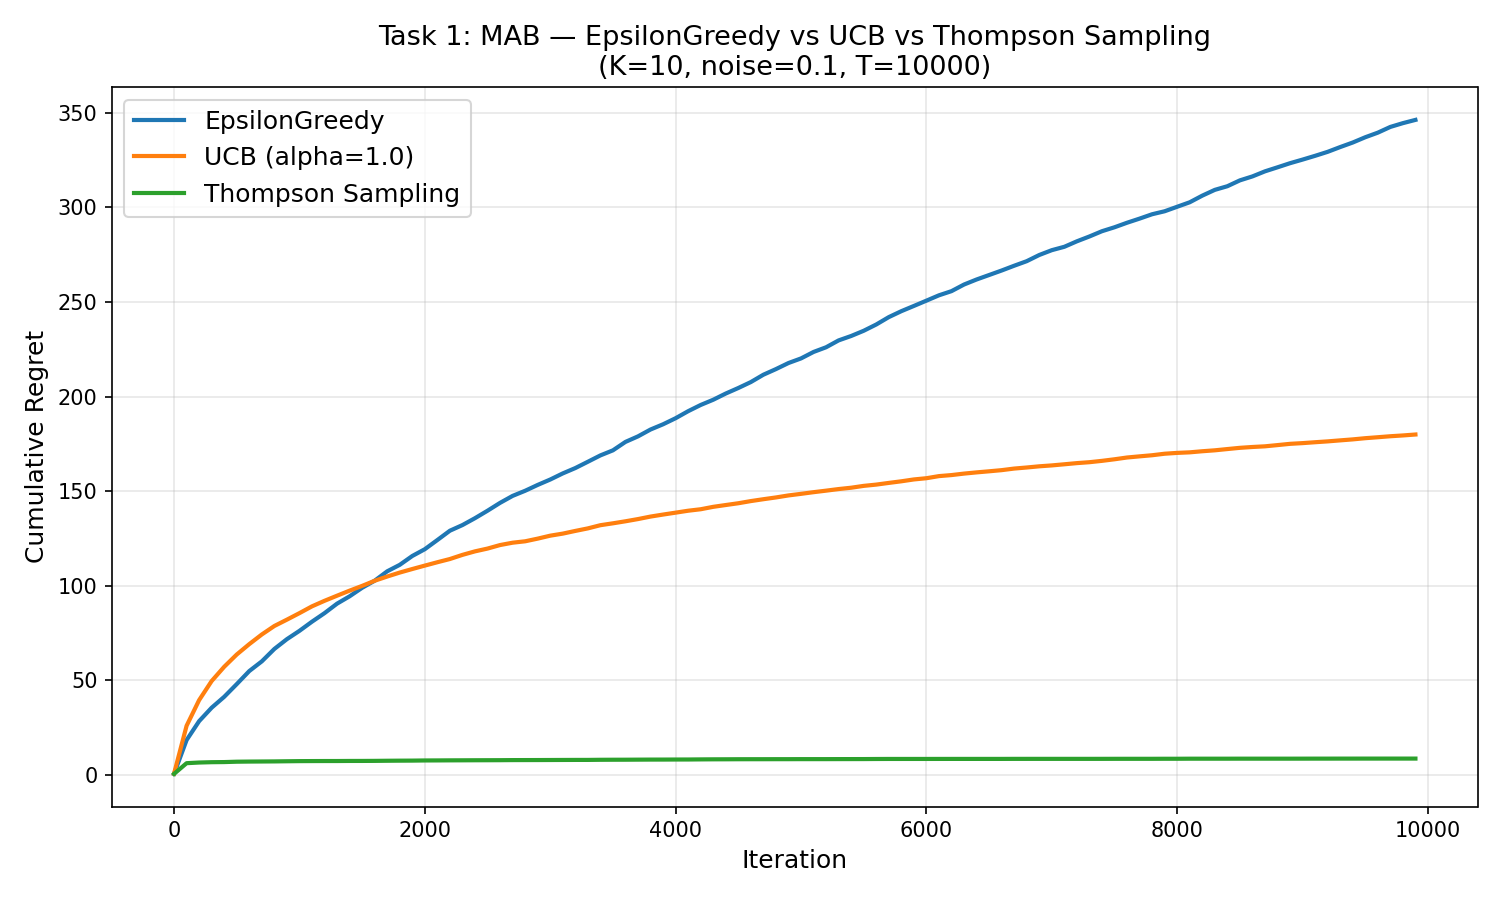
\includegraphics[width=0.85\textwidth]{SimulationResults/Task1a_MAB_comparison.png}
    \caption{MAB comparison: EpsilonGreedy vs UCB vs Thompson Sampling.}
    \label{fig:mab_compare}
\end{figure}

\begin{table}[H]
\centering
\caption{Final cumulative regret comparison for MAB algorithms.}
\begin{tabular}{cc}
\toprule
Algorithm & Final Cumulative Regret \\
\midrule
EpsilonGreedy & 346.20 \\
UCB ($\alpha = 1.0$) & 179.92 \\
\textbf{Thompson Sampling} & \textbf{8.64} \\
\bottomrule
\end{tabular}
\end{table}

Thompson Sampling dramatically outperforms both EpsilonGreedy and UCB. Its Bayesian approach naturally balances exploration and exploitation: arms with high uncertainty have wide posteriors that occasionally produce high samples (triggering exploration), while well-understood good arms consistently produce high samples (enabling exploitation). The posterior quickly concentrates around the true mean, so exploration diminishes rapidly.


% ============================================================================
% TASK 2: LINEAR BANDITS
% ============================================================================
\section{Task 2: Linear Bandits (40 points)}

\subsection{Environment Setup}

For linear bandits, we use:
\begin{itemize}[noitemsep]
    \item \texttt{actionset = "random"}: article feature vectors are random unit vectors
    \item \texttt{context\_dimension} $= d = 25$
    \item \texttt{n\_articles} $= 25$
    \item \texttt{poolArticleSize} $= 10$ (10 random articles available per round)
    \item \texttt{NoiseScale} $= \sigma = 0.1$
    \item \texttt{n\_users} $= 10$
    \item \texttt{testing\_iterations} $= 10{,}000$
\end{itemize}

The reward model is:
\[
r_t = \theta^\top x_{a_t} + \epsilon_t, \quad \epsilon_t \sim \mathcal{N}(0, \sigma^2)
\]
where $\theta \in \mathbb{R}^d$ is the user's unknown preference vector and $x_{a_t} \in \mathbb{R}^d$ is the feature vector of the selected arm. Unlike MAB, observing reward from one arm provides information about \textit{all} arms through the shared $\theta$.

% ---------- LinUCB ----------
\subsection{LinUCB (20 points)}

\subsubsection{Algorithm Description}

\textbf{Input:} Feature dimension $d$, regularization parameter $\lambda$, exploration parameter $\alpha$.

\textbf{Parameter Estimation (Ridge Regression):} We maintain:
\begin{align}
A_t &= \lambda I + \sum_{s=1}^{t} x_{a_s} x_{a_s}^\top \in \mathbb{R}^{d \times d} \label{eq:linucb_A} \\
b_t &= \sum_{s=1}^{t} x_{a_s} r_s \in \mathbb{R}^d \label{eq:linucb_b} \\
\hat{\theta}_t &= A_t^{-1} b_t \label{eq:linucb_theta}
\end{align}

\textbf{UCB for arm selection:}
\begin{equation}
\text{UCB}(x) = \hat{\theta}_t^\top x + \alpha \sqrt{x^\top A_t^{-1} x}
\label{eq:linucb}
\end{equation}

\begin{algorithm}[H]
\caption{LinUCB}
\begin{algorithmic}[1]
\State Initialize $A \leftarrow \lambda I_d$, $b \leftarrow \mathbf{0}_d$
\For{$t = 1, 2, \ldots, T$}
    \State Compute $\hat{\theta}_t = A^{-1} b$
    \For{each arm $x$ in the available set}
        \State Compute $\text{UCB}(x) = \hat{\theta}_t^\top x + \alpha \sqrt{x^\top A^{-1} x}$
    \EndFor
    \State Select $a_t = \arg\max_x \text{UCB}(x)$
    \State Observe reward $r_t$
    \State Update: $A \leftarrow A + x_{a_t} x_{a_t}^\top$, \quad $b \leftarrow b + x_{a_t} r_t$
\EndFor
\end{algorithmic}
\end{algorithm}

The term $\sqrt{x^\top A_t^{-1} x}$ measures the uncertainty of the predicted reward in the direction $x$. Directions that have been observed frequently contribute more to $A_t$, reducing uncertainty in those directions.

\textbf{Hyperparameters used:} $\lambda = 1.0$, $\alpha \in \{0.1, 0.5, 1.0\}$.

\subsubsection{Results}

\begin{figure}[H]
    \centering
    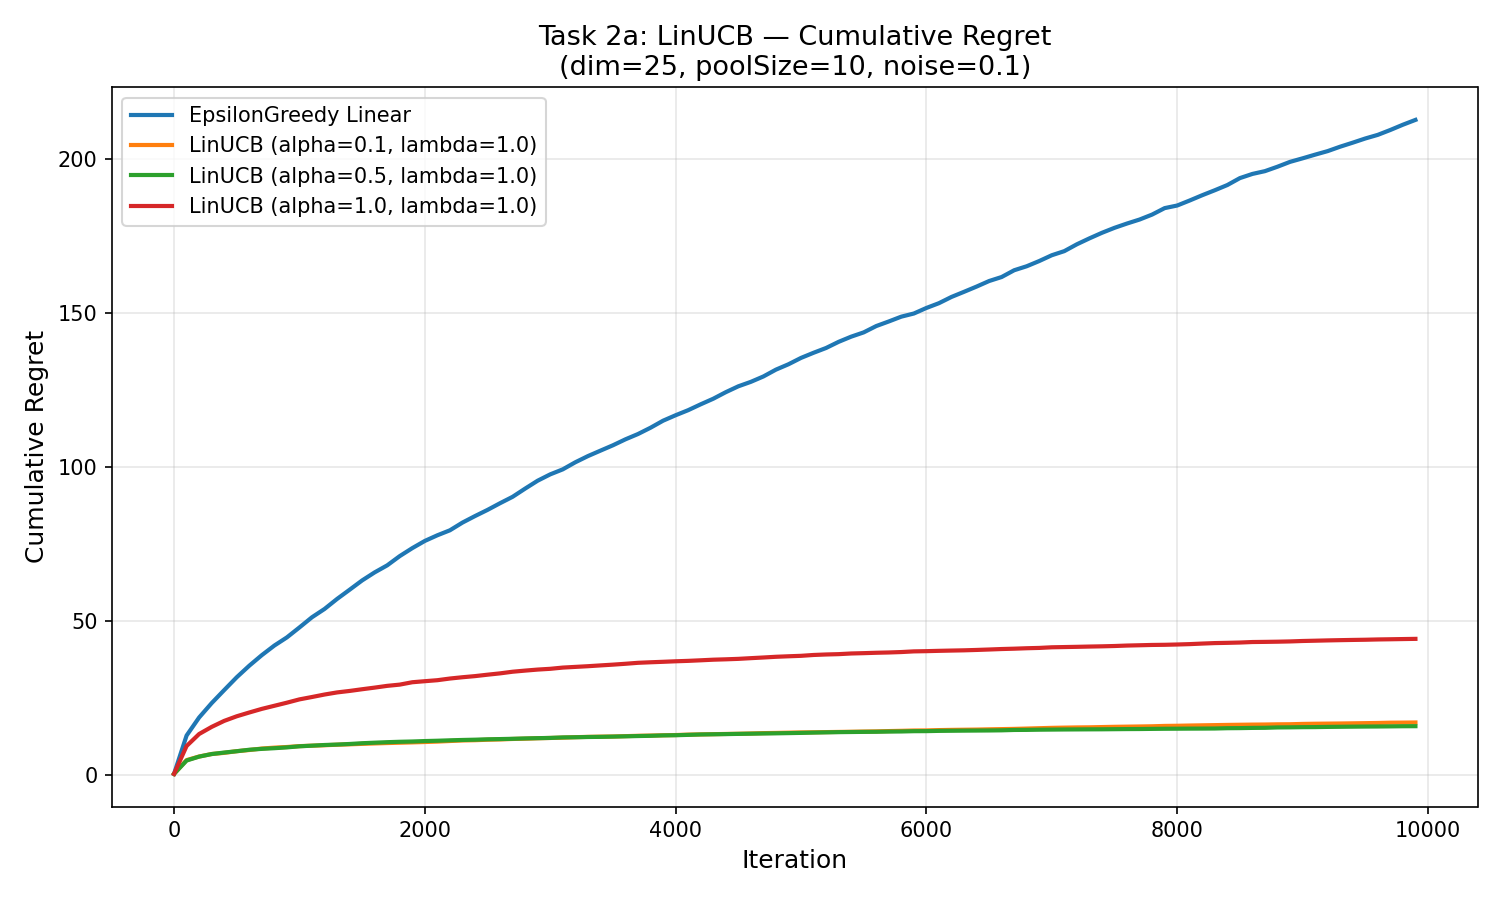
\includegraphics[width=0.85\textwidth]{SimulationResults/Task2a_LinUCB_regret.png}
    \caption{LinUCB: Cumulative regret with different $\alpha$ values.}
    \label{fig:linucb_regret}
\end{figure}

\begin{figure}[H]
    \centering
    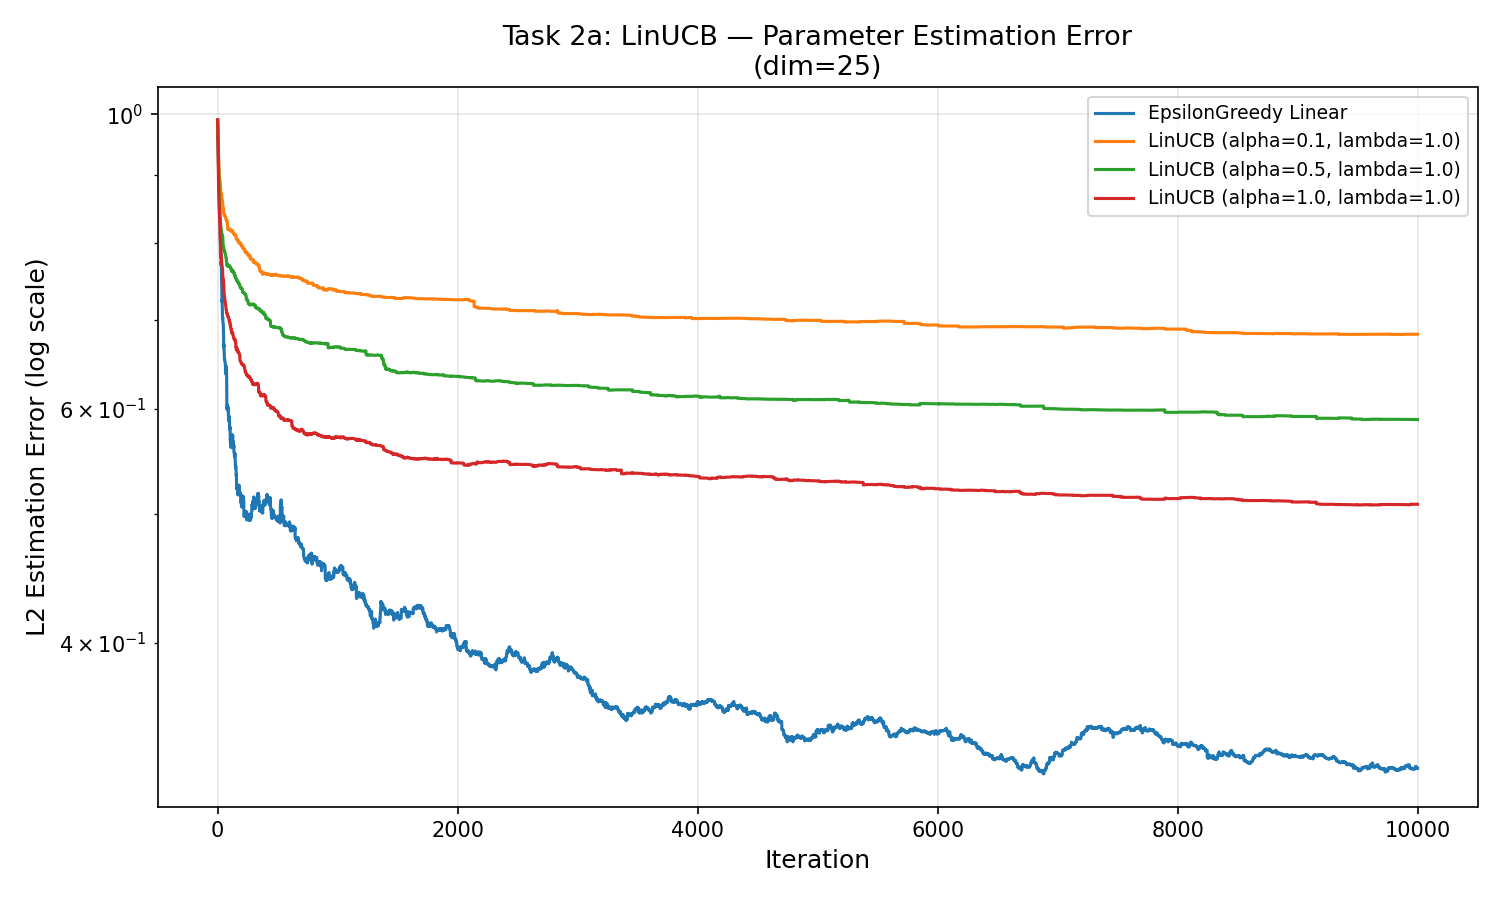
\includegraphics[width=0.85\textwidth]{SimulationResults/Task2a_LinUCB_theta_error.png}
    \caption{LinUCB: Parameter estimation error $\|\theta - \hat{\theta}\|_2$ over time (log scale).}
    \label{fig:linucb_theta}
\end{figure}

\begin{table}[H]
\centering
\caption{LinUCB final cumulative regret.}
\begin{tabular}{ccc}
\toprule
$\alpha$ & $\lambda$ & Final Cumulative Regret \\
\midrule
0.1 & 1.0 & 16.93 \\
\textbf{0.5} & \textbf{1.0} & \textbf{15.73} \\
1.0 & 1.0 & 44.11 \\
\midrule
\multicolumn{2}{c}{EpsilonGreedy Linear} & 212.80 \\
\bottomrule
\end{tabular}
\end{table}

LinUCB with $\alpha = 0.5$ achieves the best performance. The parameter estimation error decreases steadily over time as $A_t$ accumulates more observations, and LinUCB dramatically outperforms EpsilonGreedy by leveraging the linear structure of the reward function.

% ---------- LinTS ----------
\subsection{LinTS (20 points)}

\subsubsection{Algorithm Description}

\textbf{Input:} Feature dimension $d$, regularization parameter $\lambda$, sampling scale $v$.

Linear Thompson Sampling uses the same ridge regression as LinUCB but replaces the confidence bound with posterior sampling.

\textbf{Prior:}
\[
\theta \sim \mathcal{N}\left(\mathbf{0}, \frac{1}{\lambda} I_d\right)
\]

\textbf{Posterior} after $t$ observations:
\begin{align}
\theta \mid \text{data} &\sim \mathcal{N}(\mu_t, V_t) \\
V_t &= A_t^{-1} = \left(\lambda I + \sum_{s=1}^{t} x_{a_s} x_{a_s}^\top\right)^{-1} \label{eq:lints_V} \\
\mu_t &= V_t b_t = A_t^{-1} \sum_{s=1}^{t} x_{a_s} r_s \label{eq:lints_mu}
\end{align}

\textbf{Decision:}
\begin{align}
\tilde{\theta}_t &\sim \mathcal{N}(\mu_t, v^2 V_t) \label{eq:lints_sample} \\
a_t &= \arg\max_{x \in \mathcal{A}_t} \tilde{\theta}_t^\top x \label{eq:lints_decision}
\end{align}

\begin{algorithm}[H]
\caption{LinTS}
\begin{algorithmic}[1]
\State Initialize $A \leftarrow \lambda I_d$, $b \leftarrow \mathbf{0}_d$
\For{$t = 1, 2, \ldots, T$}
    \State Compute $\mu_t = A^{-1} b$ and $V_t = A^{-1}$
    \State Sample $\tilde{\theta}_t \sim \mathcal{N}(\mu_t, v^2 V_t)$
    \State Select $a_t = \arg\max_x \tilde{\theta}_t^\top x$
    \State Observe reward $r_t$
    \State Update: $A \leftarrow A + x_{a_t} x_{a_t}^\top$, \quad $b \leftarrow b + x_{a_t} r_t$
\EndFor
\end{algorithmic}
\end{algorithm}

The parameter $v$ controls the amount of exploration: theoretically $v^2 = \sigma^2$, but in practice it can be tuned.

\textbf{Hyperparameters used:} $\lambda = 1.0$, $\sigma = 0.1$, $v \in \{0.01, 0.1, 0.5\}$.

\subsubsection{Results}

\begin{figure}[H]
    \centering
    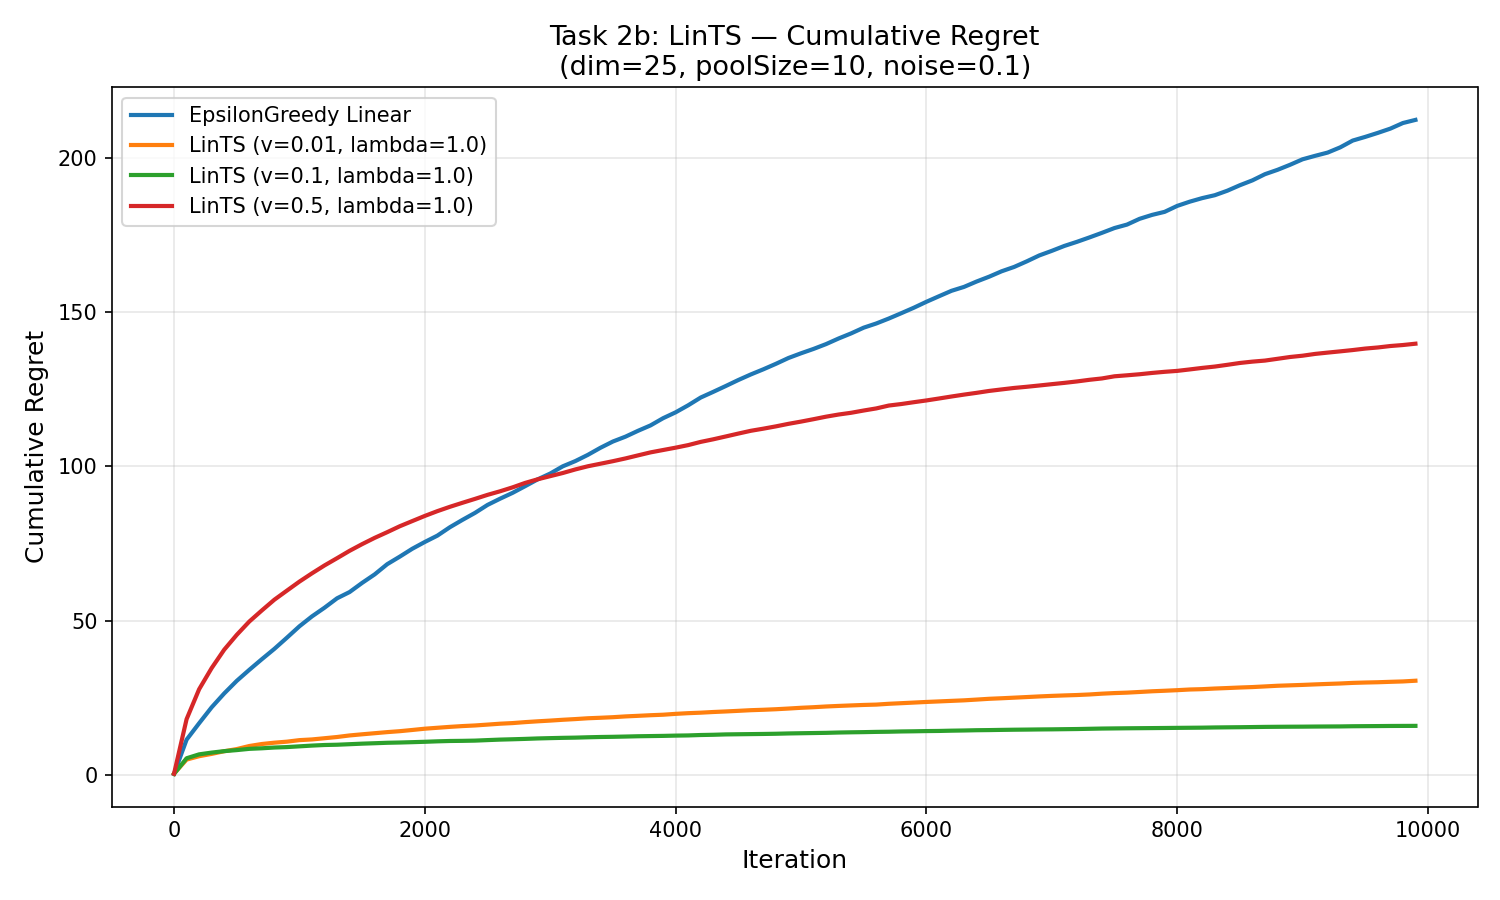
\includegraphics[width=0.85\textwidth]{SimulationResults/Task2b_LinTS_regret.png}
    \caption{LinTS: Cumulative regret with different $v$ values.}
    \label{fig:lints_regret}
\end{figure}

\begin{figure}[H]
    \centering
    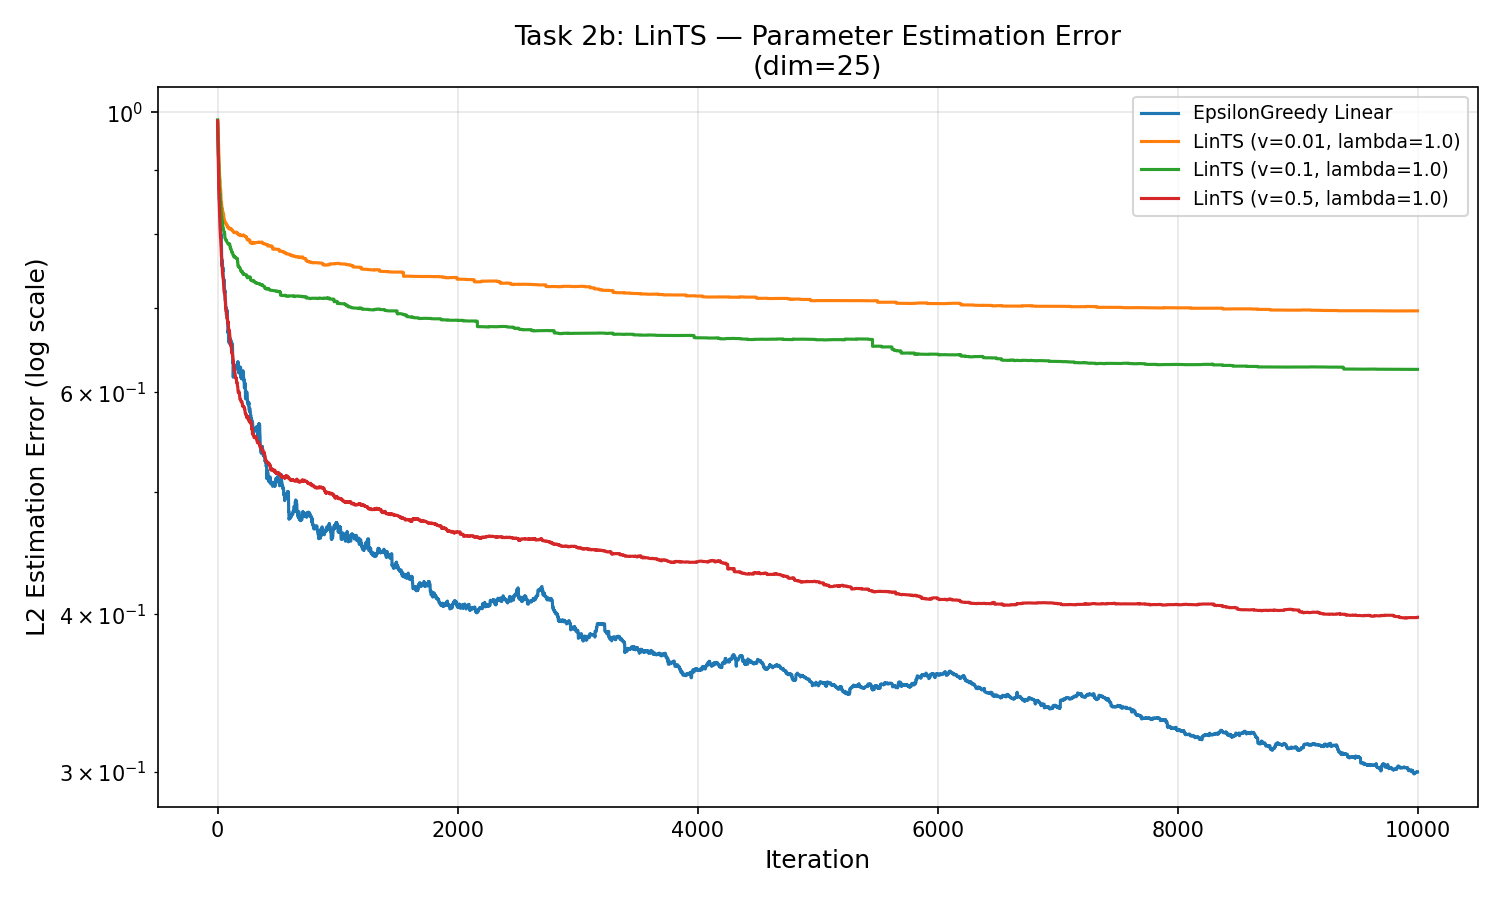
\includegraphics[width=0.85\textwidth]{SimulationResults/Task2b_LinTS_theta_error.png}
    \caption{LinTS: Parameter estimation error over time (log scale).}
    \label{fig:lints_theta}
\end{figure}

\begin{table}[H]
\centering
\caption{LinTS final cumulative regret.}
\begin{tabular}{cccc}
\toprule
$v$ & $\lambda$ & $\sigma$ & Final Cumulative Regret \\
\midrule
0.01 & 1.0 & 0.1 & 30.49 \\
\textbf{0.1} & \textbf{1.0} & \textbf{0.1} & \textbf{15.86} \\
0.5 & 1.0 & 0.1 & 139.70 \\
\midrule
\multicolumn{3}{c}{EpsilonGreedy Linear} & 212.23 \\
\bottomrule
\end{tabular}
\end{table}

$v = 0.1 = \sigma$ (matching the noise standard deviation) gives the best performance, consistent with theory. When $v$ is too small ($v=0.01$), the algorithm under-explores and converges slowly. When $v$ is too large ($v=0.5$), it over-explores.

% ---------- Combined Comparison ----------
\subsection{Combined Comparison: LinUCB vs LinTS vs EpsilonGreedy}

\begin{figure}[H]
    \centering
    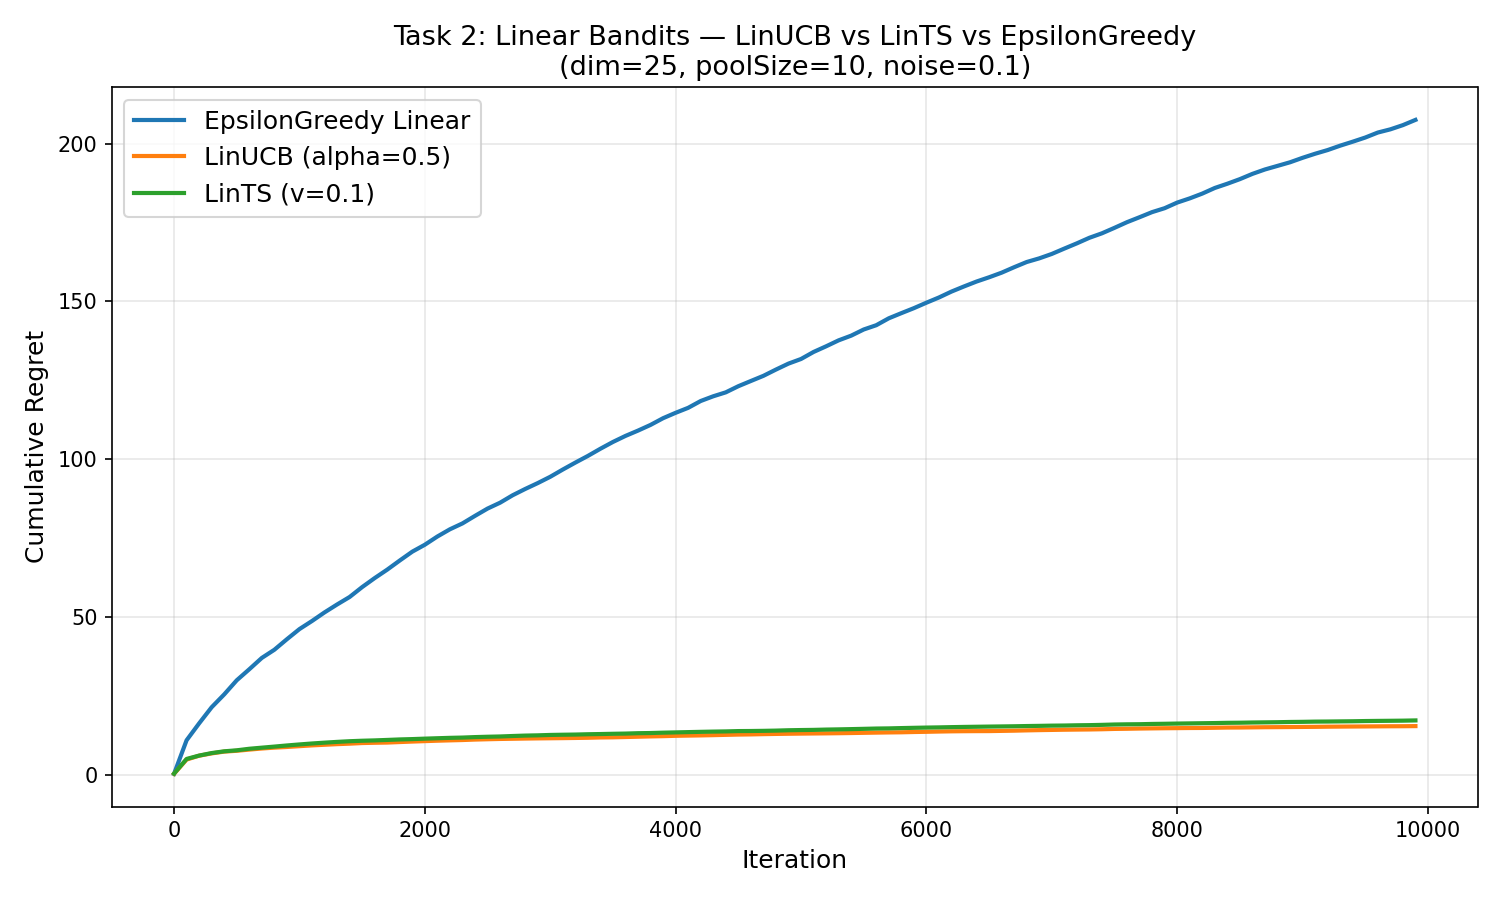
\includegraphics[width=0.85\textwidth]{SimulationResults/Task2c_Linear_comparison.png}
    \caption{Linear bandits: LinUCB vs LinTS vs EpsilonGreedy cumulative regret.}
    \label{fig:linear_compare}
\end{figure}

\begin{figure}[H]
    \centering
    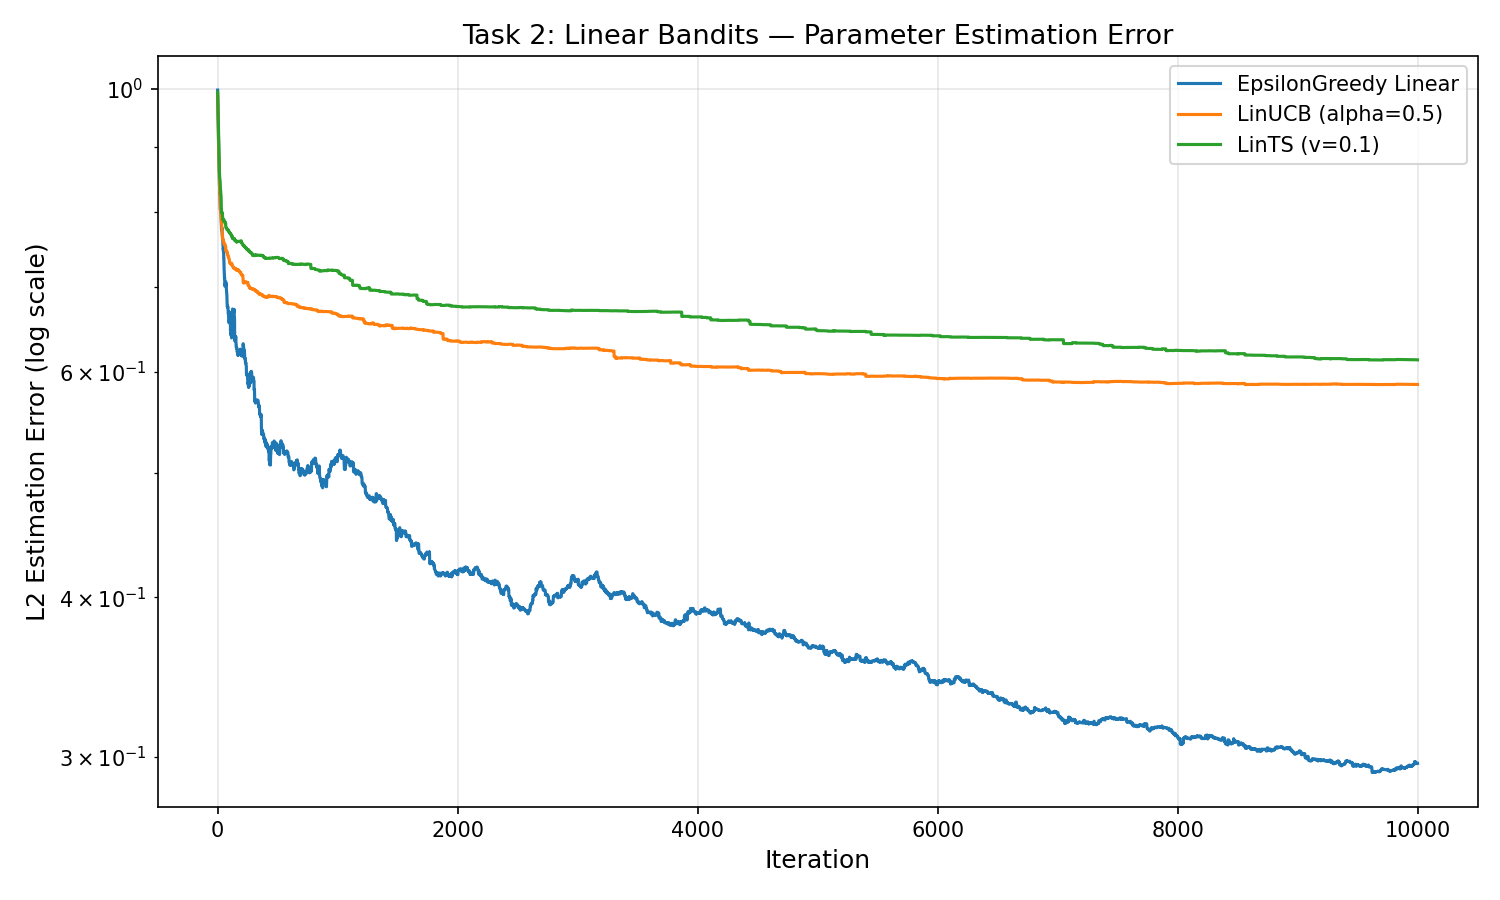
\includegraphics[width=0.85\textwidth]{SimulationResults/Task2c_Linear_theta_error.png}
    \caption{Linear bandits: Parameter estimation error comparison.}
    \label{fig:linear_theta}
\end{figure}

\begin{table}[H]
\centering
\caption{Final comparison of linear bandit algorithms.}
\begin{tabular}{cc}
\toprule
Algorithm & Final Cumulative Regret \\
\midrule
EpsilonGreedy Linear & 207.52 \\
\textbf{LinUCB ($\alpha=0.5$)} & \textbf{15.40} \\
LinTS ($v=0.1$) & 17.21 \\
\bottomrule
\end{tabular}
\end{table}

Both LinUCB and LinTS significantly outperform EpsilonGreedy (by more than $10\times$). LinUCB and LinTS achieve comparable performance. The parameter estimation error (Figure~\ref{fig:linear_theta}) decreases over time for all algorithms, confirming that the ridge regression estimator converges to the true $\theta$.

% ============================================================================
% CONCLUSION
% ============================================================================
\section{Conclusion}

Key takeaways from the experiments:

\begin{enumerate}
    \item \textbf{Explore Then Commit} has a clear exploration-exploitation tradeoff controlled by $m$. The optimal $m$ depends on the noise level and time horizon. It is simple but inflexible compared to adaptive methods.
    
    \item \textbf{UCB} adaptively balances exploration and exploitation through confidence bounds. It achieves $O(\sqrt{K \ln T})$ regret and requires no distributional assumptions.
    
    \item \textbf{Thompson Sampling} is the best-performing MAB algorithm, achieving near-optimal regret. Its Bayesian nature provides a natural and effective exploration mechanism.
    
    \item \textbf{LinUCB and LinTS} leverage the linear reward structure to share information across arms, achieving dramatically lower regret than MAB baselines in the linear setting. Both achieve comparable performance, with LinUCB being slightly deterministic and LinTS being stochastic.
\end{enumerate}

% ============================================================================
% REFERENCES
% ============================================================================
\begin{thebibliography}{1}
\bibitem{lattimore2020} T. Lattimore and C. Szepesv\'{a}ri. \textit{Bandit Algorithms}. Cambridge University Press, 2020.
\end{thebibliography}

\end{document}
